\section{Foundations and Model A: steady populations under a fixed catch}
\label{sec:foundations}

\paragraph{Question.} Suppose the same amount is caught every year. At what population sizes can the stock hold steady, which of these are safe, and how large can the catch be before collapse becomes certain?

\subsection{Scaling}
\label{sec:scaling}
The model has four parameters, but only two combinations of them actually matter. If we measure the population as a fraction of capacity, $x=N/K$, and time in units of $1/r$, $\tau=rt$, the chain rule gives $dN/dt=rK\,dx/d\tau$. Dividing Eq.~\eqref{eq:modelA} by $rK$ then leaves
\begin{equation}
\frac{dx}{d\tau}=f(x)=G(x)-q,\qquad G(x)=x(1-x)\Bigl(\frac{x}{a}-1\Bigr),
\label{eq:A_dimless}
\end{equation}
where $a=A/K$ is the Allee threshold as a fraction of capacity and $q=H/(rK)$ is the scaled catch. In the same way the logistic model becomes $dx/d\tau=x(1-x)-q$, and Model B becomes $dx/d\tau=G(x)-ex$ with $e=h/r$. Any result can be turned back into real units using $N=Kx$, $t=\tau/r$ and $H=rKq$. All examples in this section use $a=0.2$.

\subsection{Steady states and stability}
A steady state, or equilibrium, is a population $x_e$ at which growth and catch cancel out, so that $f(x_e)=0$ and nothing changes. To decide whether it is stable, we look at the sign of $f$ just on either side of it \cite{strogatz2015nonlinear}. If $f$ is positive just below $x_e$ and negative just above, a population nudged slightly away is pulled back, and the state is \emph{stable}. If the signs are the other way round, small nudges grow and the state is \emph{unstable}. If $f$ has the same sign on both sides, the state attracts from one side and repels on the other, and we call it \emph{semistable}. Wherever $f'(x_e)\neq0$ this agrees with the familiar derivative test ($f'<0$ stable, $f'>0$ unstable), but at a point where $f'(x_e)=0$ only the signs can settle the question.

\paragraph{Logistic baseline.} It helps to start with the model without an Allee effect, $f(x)=x(1-x)-q$. For $q<\tfrac14$ it has two steady states,
\begin{equation}
x_\pm=\tfrac12\bigl(1\pm\sqrt{1-4q}\bigr).
\end{equation}
The upper one is stable. The lower one is unstable, a threshold that exists only because of the catch. As $q$ grows the two move towards each other and meet at $x=\tfrac12$ when $q=\tfrac14$, which gives the well-known maximum constant catch $H_c=rK/4$ \cite{brauer2012mathematical}. Any larger catch drives every population to zero. With no catch at all, zero is unstable, so even a very small population grows back.

\subsection{Model A: the growth curve and the maximum catch}
With the Allee factor included, the growth curve $G$ is negative between $0$ and $a$ and positive between $a$ and $1$. In other words, it dips below zero when the population is small and then rises into a single hill. The top of the hill is where $G'(x)=0$, which works out to $3x^2-2(1+a)x+a=0$. Taking the larger root,
\begin{equation}
x^*=\frac{1+a+\sqrt{1-a+a^2}}{3},\qquad q_c=G(x^*).
\label{eq:fold}
\end{equation}
Steady states are the points where the horizontal line at height $q$ meets this curve, which leaves four cases.
\begin{itemize}
\item With no catch ($q=0$) there are three steady states. Both $x=0$ and $x=1$ are stable, while $x=a$ in between is unstable: this is the minimum viable population. Unlike the logistic model, extinction is now a stable outcome.
\item For a moderate catch ($0<q<q_c$) the line cuts the hill twice, at an unstable $x_-$ between $a$ and $x^*$ and a stable $x_+$ between $x^*$ and $1$. A population starting below $x_-$ dies out, while one starting above it settles at $x_+$.
\item At $q=q_c$ the line just touches the top of the hill, and the two states merge into a single semistable point at $x^*$, called the \emph{fold}.
\item For $q>q_c$ the line never meets the hill, and every population collapses.
\end{itemize}

Once there is any catch at all, zero stops being a steady state, because $f(0)=-q<0$. A declining population therefore reaches zero in finite time, and we stop the simulation at that point. For $a=0.2$ we get $x^*\approx0.706$ and $q_c\approx0.525$. With $r=0.5$ per year and $K=1000$ t, the largest catch the stock can sustain is about $263$ t/yr, at a stock of about $706$ t.

\subsection{Finding the steady states numerically}
To compute the steady states for a given catch, we use the shape of $G$ directly:
\begin{enumerate}
\item Compute $x^*$ and $q_c$ from Eq.~\eqref{eq:fold}.
\item If $q>q_c$ there is no positive steady state, and if $q=q_c$ the only one is $x^*$.
\item If $0<q<q_c$, $f$ changes sign exactly once between $a$ and $x^*$ and once between $x^*$ and $1$. Each root is found with Brent's method, a standard root finder that repeatedly shrinks an interval containing a sign change.
\item Each root is then labelled stable or unstable from the sign of $f$ on either side.
\end{enumerate}
For $a=0.2$ and $q=0.3$ this gives $x_-=0.4431$ (unstable) and $x_+=0.9063$ (stable). Very close to $q_c$ the two roots become nearly equal, and if floating-point arithmetic cannot tell them apart, the code reports an error instead of quietly merging them.

\subsection{Growth curves and the branch diagram}
Figure~\ref{fig:wp01_geometry} puts this picture on paper. In the logistic panels a threshold only appears once fishing starts. Model A already has one at $x=a$ with no catch, and fishing pushes it higher. Once the catch exceeds $q_c$, the line passes above the whole hill.

\begin{figure}[!htbp]
\centering
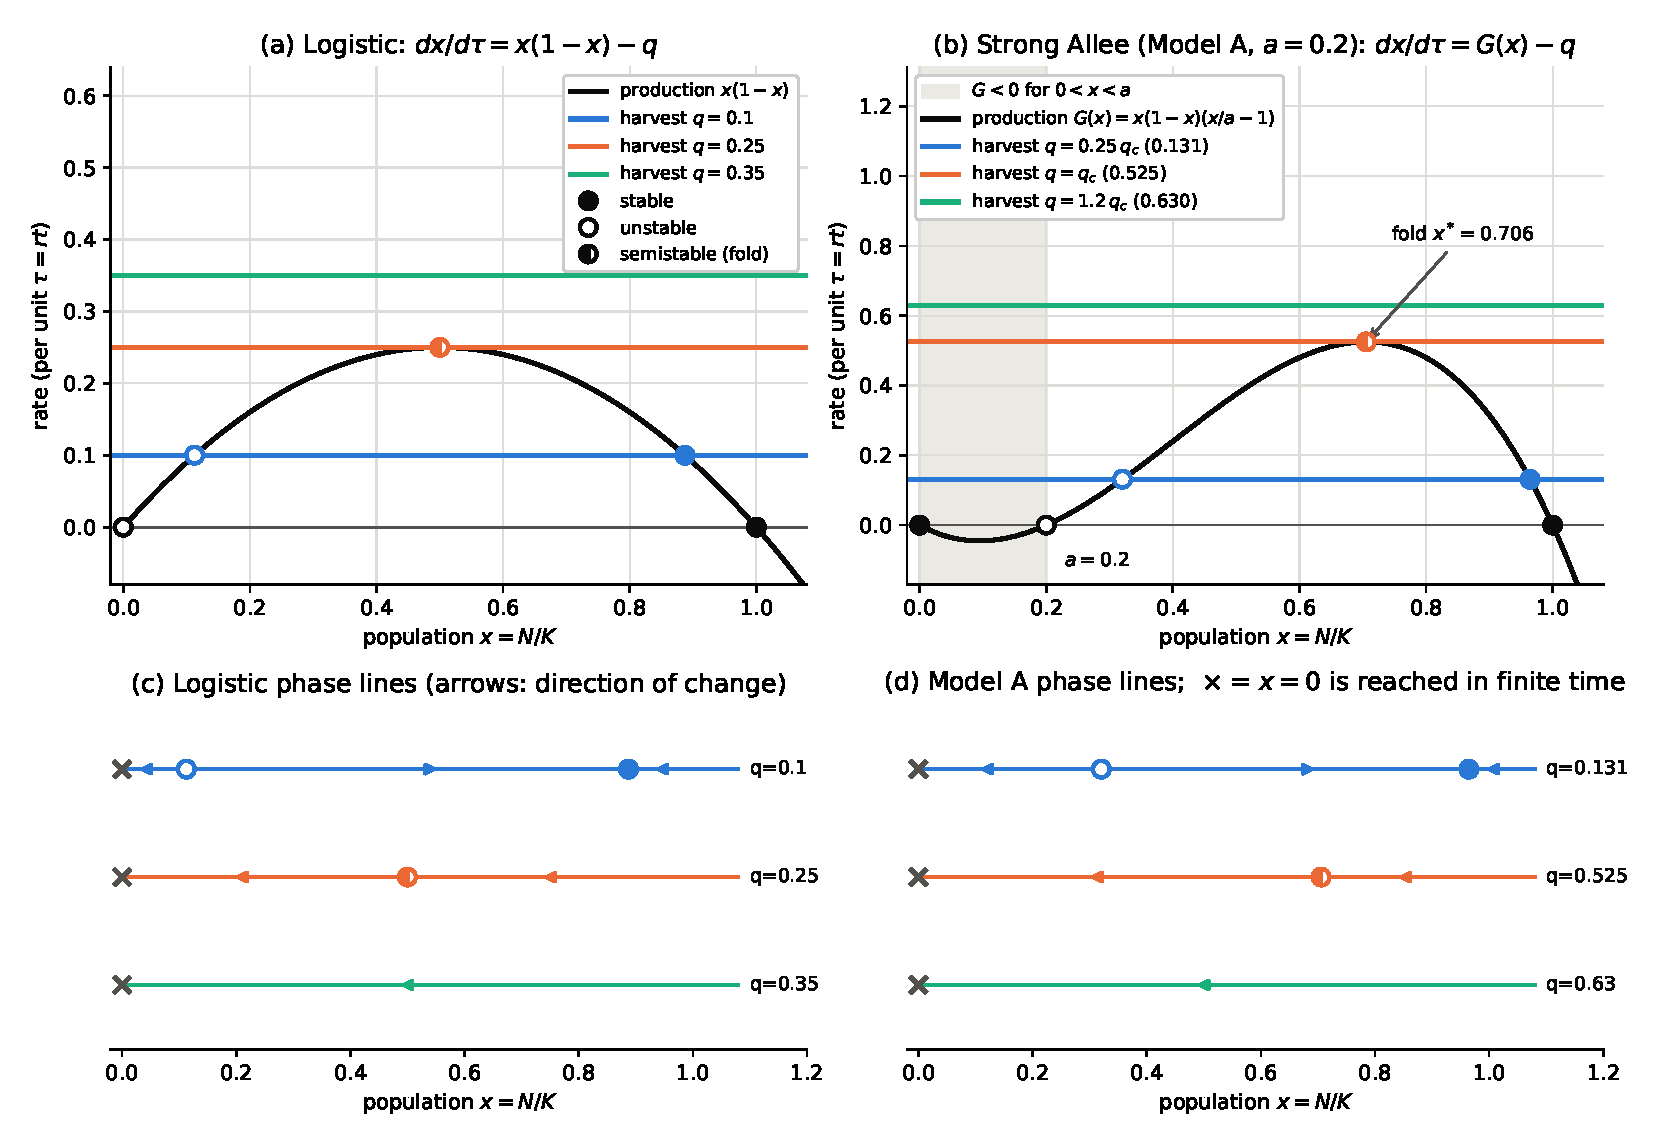
\includegraphics[width=0.85\textwidth]{wp01_logistic_vs_allee}
\caption{Growth curves and phase lines. (a)~Logistic growth $x(1-x)$ with catch lines. (b)~Strong-Allee growth $G(x)$ for $a=0.2$, with catches of $0.25q_c$, $q_c$ and $1.2q_c$. Filled, open and half-filled circles mark stable, unstable and semistable states. (c,d)~Phase lines: arrows show whether the population grows or shrinks, and $\times$ marks $x=0$, which is reached in finite time when $q>0$.}
\label{fig:wp01_geometry}
\end{figure}

Plotting the steady states against the catch gives the branch diagram in Figure~\ref{fig:wp01_branches}. As the catch increases, the stable branch and the collapse threshold approach each other and meet at the fold $(q_c,x^*)$. The distance $x_+-x_-$ between them is the stock's safety margin, and near the fold it shrinks like $\sqrt{q_c-q}$.

\begin{figure}[!htbp]
\centering
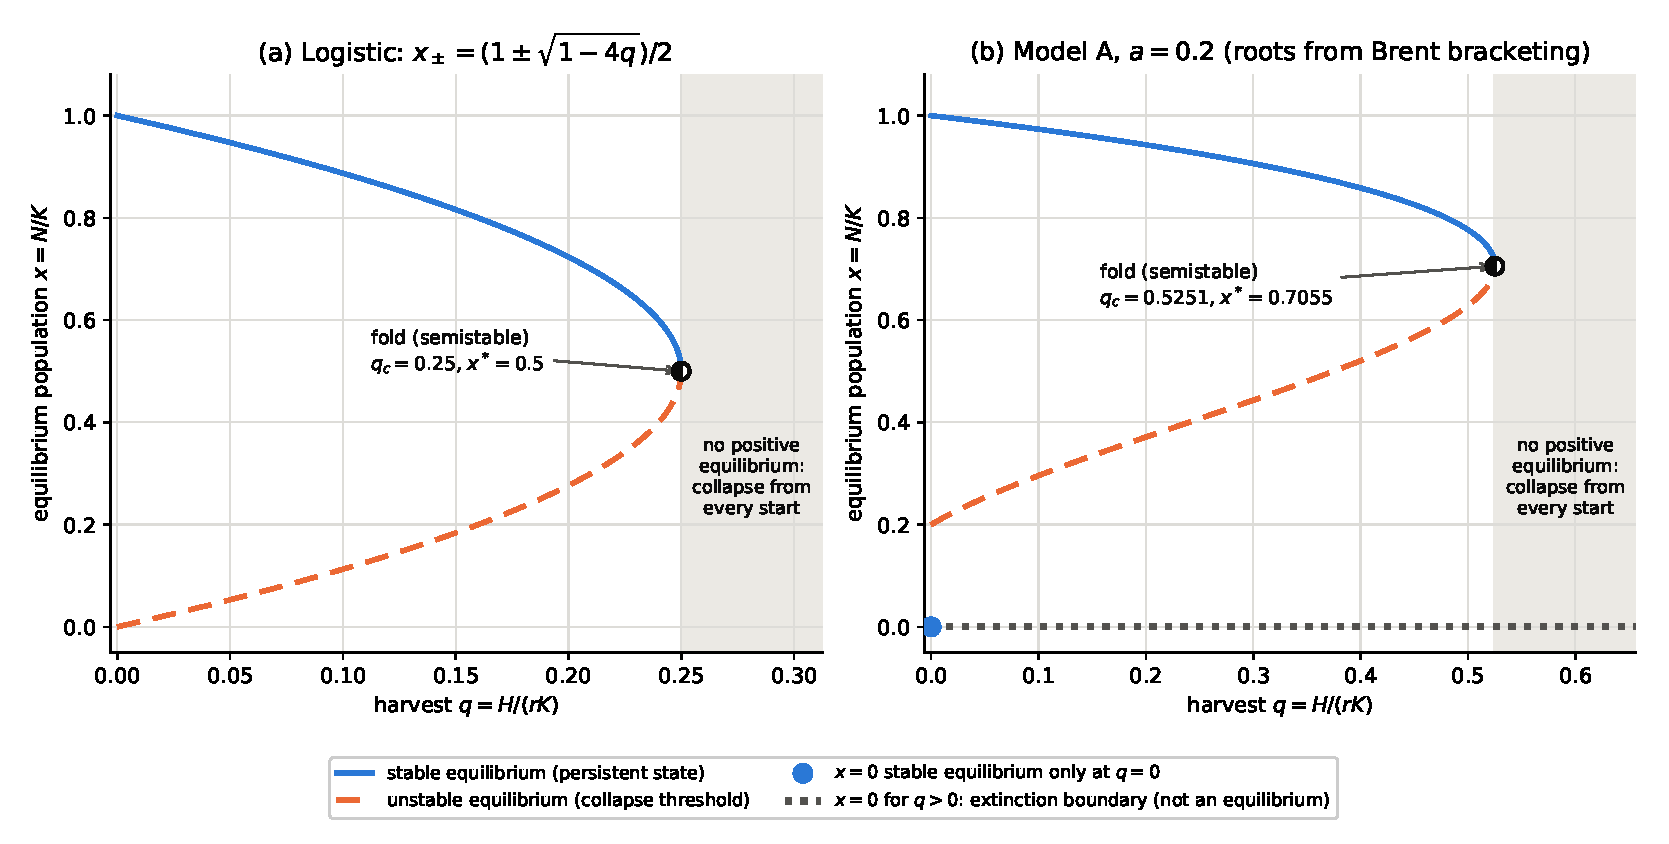
\includegraphics[width=0.92\textwidth]{wp01_model_a_branches}
\caption{Steady states against the scaled catch $q=H/(rK)$. (a)~Logistic. (b)~Model A with $a=0.2$. Solid lines are stable, dashed lines unstable, and the half-filled circle is the semistable fold. The shaded region $q>q_c$ has no positive steady state. In (b) the dotted line at $x=0$ marks extinction, which is not a steady state when $q>0$.}
\label{fig:wp01_branches}
\end{figure}

\subsection{Checking stability by simulation}
As a check on these labels, we took $q=0.3$, started the population $\delta=0.01$ above and below each steady state, and solved the equation with a standard Runge--Kutta solver (RK45 \cite{scipy_solve_ivp}) that stops at $x=0$. Both starts near $x_+$ return to it. The start just above $x_-$ climbs back up to $x_+$, while the one just below falls and reaches zero at $\tau\approx2.9$ (Figure~\ref{fig:wp01_perturb}). This is exactly what the sign analysis predicted.

\begin{figure}[!htbp]
\centering
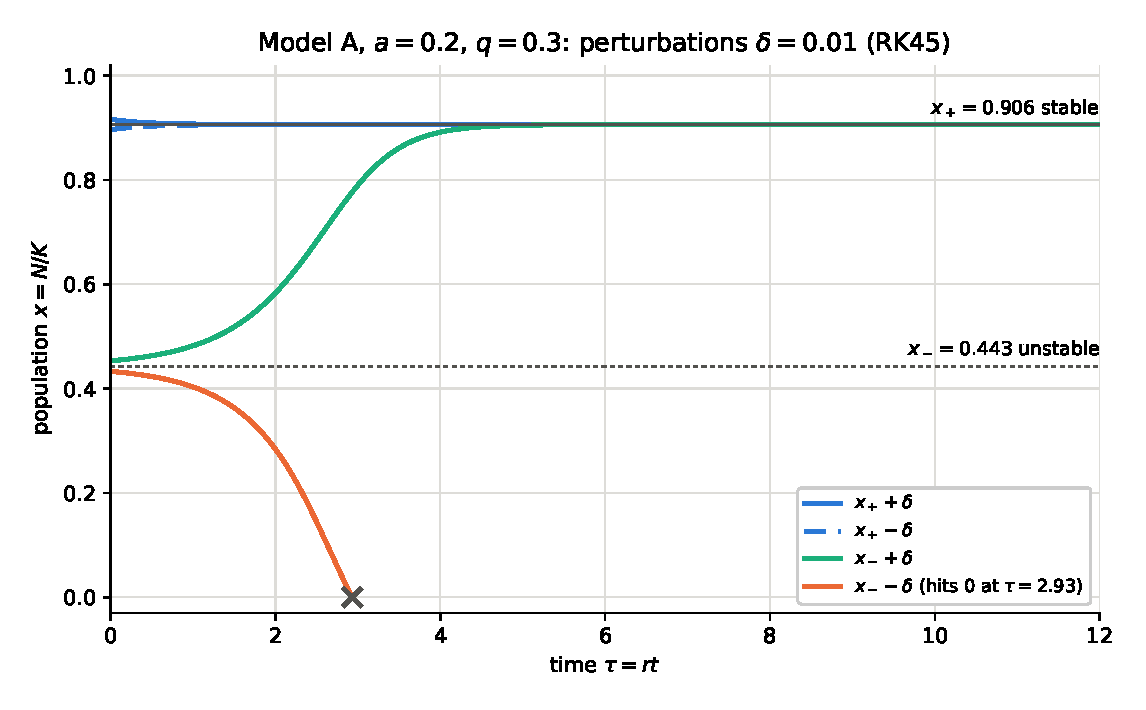
\includegraphics[width=0.62\textwidth]{wp01_model_a_perturbations}
\caption{Simulation check for Model A with $a=0.2$ and $q=0.3$, starting $\delta=0.01$ above and below each steady state.}
\label{fig:wp01_perturb}
\end{figure}

\FloatBarrier
\subsection{Result and limitations}
\paragraph{Main result.} As the fixed catch rises, the safe steady state and the collapse threshold draw closer and finally merge at the maximum catch $q_c$. A disturbance only causes collapse if it pushes the population below the threshold, that is, if it is larger than the gap between the two. Since this gap closes at $q_c$, fishing near the maximum leaves almost no room for a bad year.

\paragraph{Limitations.} The model ignores randomness, which matters most near the threshold. The cubic growth law is a simple phenomenological choice, the parameters are held constant, and the full catch is assumed to be taken whenever $N>0$. All numbers are illustrative rather than measured from a real stock.